\documentclass[10pt]{dokument-ppi}

\begin{document}


\Cwiczenie{3}
\Tytul{Harmonogram pracy}
\Data{2012-12-04}
\Autorzy{TC, MM, MO, ŁG, DG, AO, MS}
\MakeDokumentMeta


\section{Harmonogram pracy}

\subsection{Iteracja A -- Przygotowanie}

Harmonogram prac wchodzących w skład iteracji \emph{Przygotowanie}
zaczyna się na stronie \pageref{fig:iteracja-przygotowanie}.

\begin{figure}[p]
    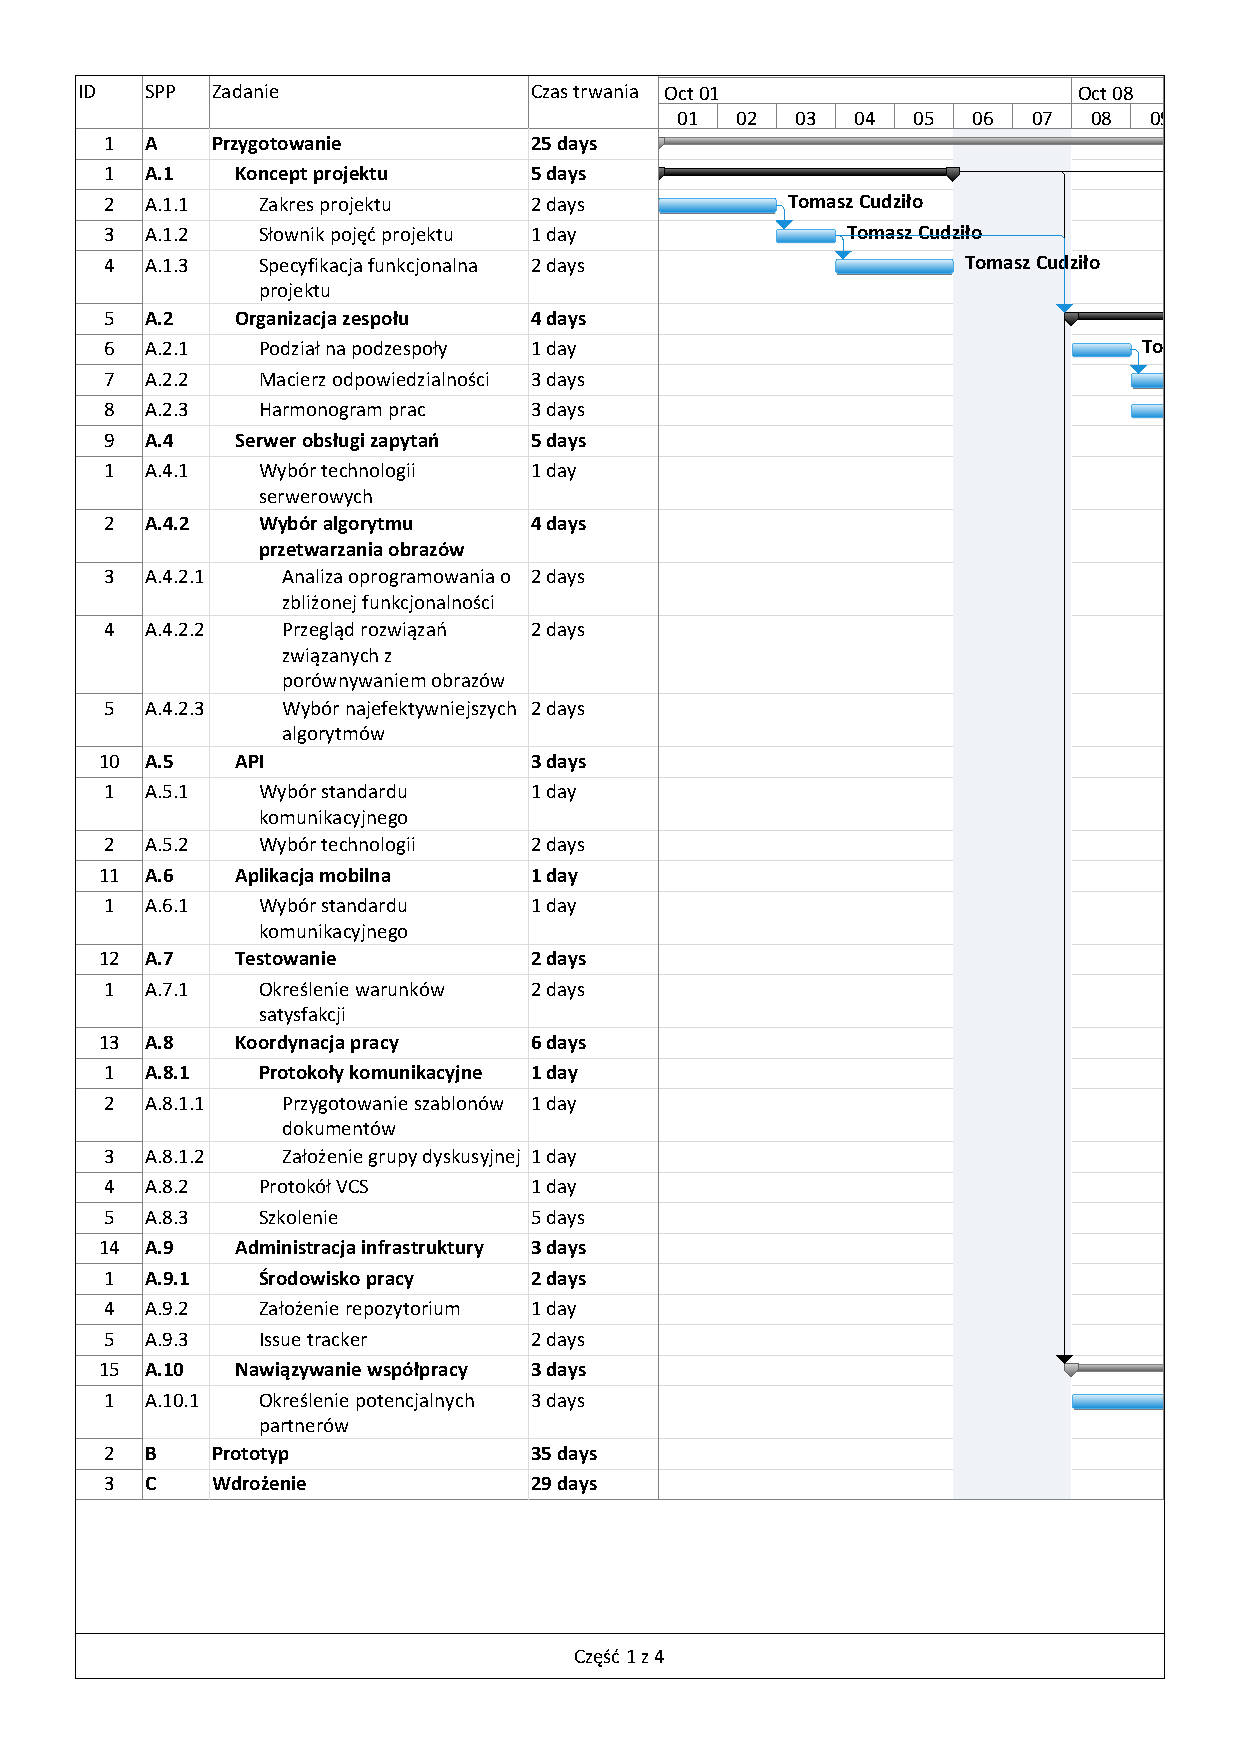
\includegraphics[trim=1.2cm 1.2cm 1.2cm 1.2cm,page=1,width=\textwidth]{./figury/organizacja-pracy-A-przygotowanie}
    \caption{Harmonogram pracy iteracji \emph{Przygotowanie} projektu \emph{Concerto}.}
    \label{fig:iteracja-przygotowanie}
\end{figure}

\begin{figure}[p]
    \ContinuedFloat
    \includegraphics[trim=1.2cm 1.2cm 1.2cm 1.2cm,page=2,width=\textwidth]{./figury/organizacja-pracy-A-przygotowanie}
    \caption[]{Harmonogram pracy iteracji \emph{Przygotowanie} projektu \emph{Concerto}. (kontynuacja)}
\end{figure}

\begin{figure}[p]
    \ContinuedFloat
    \includegraphics[trim=1.2cm 1.2cm 1.2cm 1.2cm,page=3,width=\textwidth]{./figury/organizacja-pracy-A-przygotowanie}
    \caption[]{Harmonogram pracy iteracji \emph{Przygotowanie} projektu \emph{Concerto}. (kontynuacja)}
\end{figure}

\begin{figure}[p]
    \ContinuedFloat
    \includegraphics[trim=1.2cm 1.2cm 1.2cm 1.2cm,page=4,width=\textwidth]{./figury/organizacja-pracy-A-przygotowanie}
    \caption[]{Harmonogram pracy iteracji \emph{Przygotowanie} projektu \emph{Concerto}. (kontynuacja)}
\end{figure}

\subsection{Iteracja B -- Prototyp}

Harmonogram prac wchodzących w skład iteracji \emph{Prototyp}
zaczyna się na stronie \pageref{fig:iteracja-prototyp}.

\begin{figure}[p]
    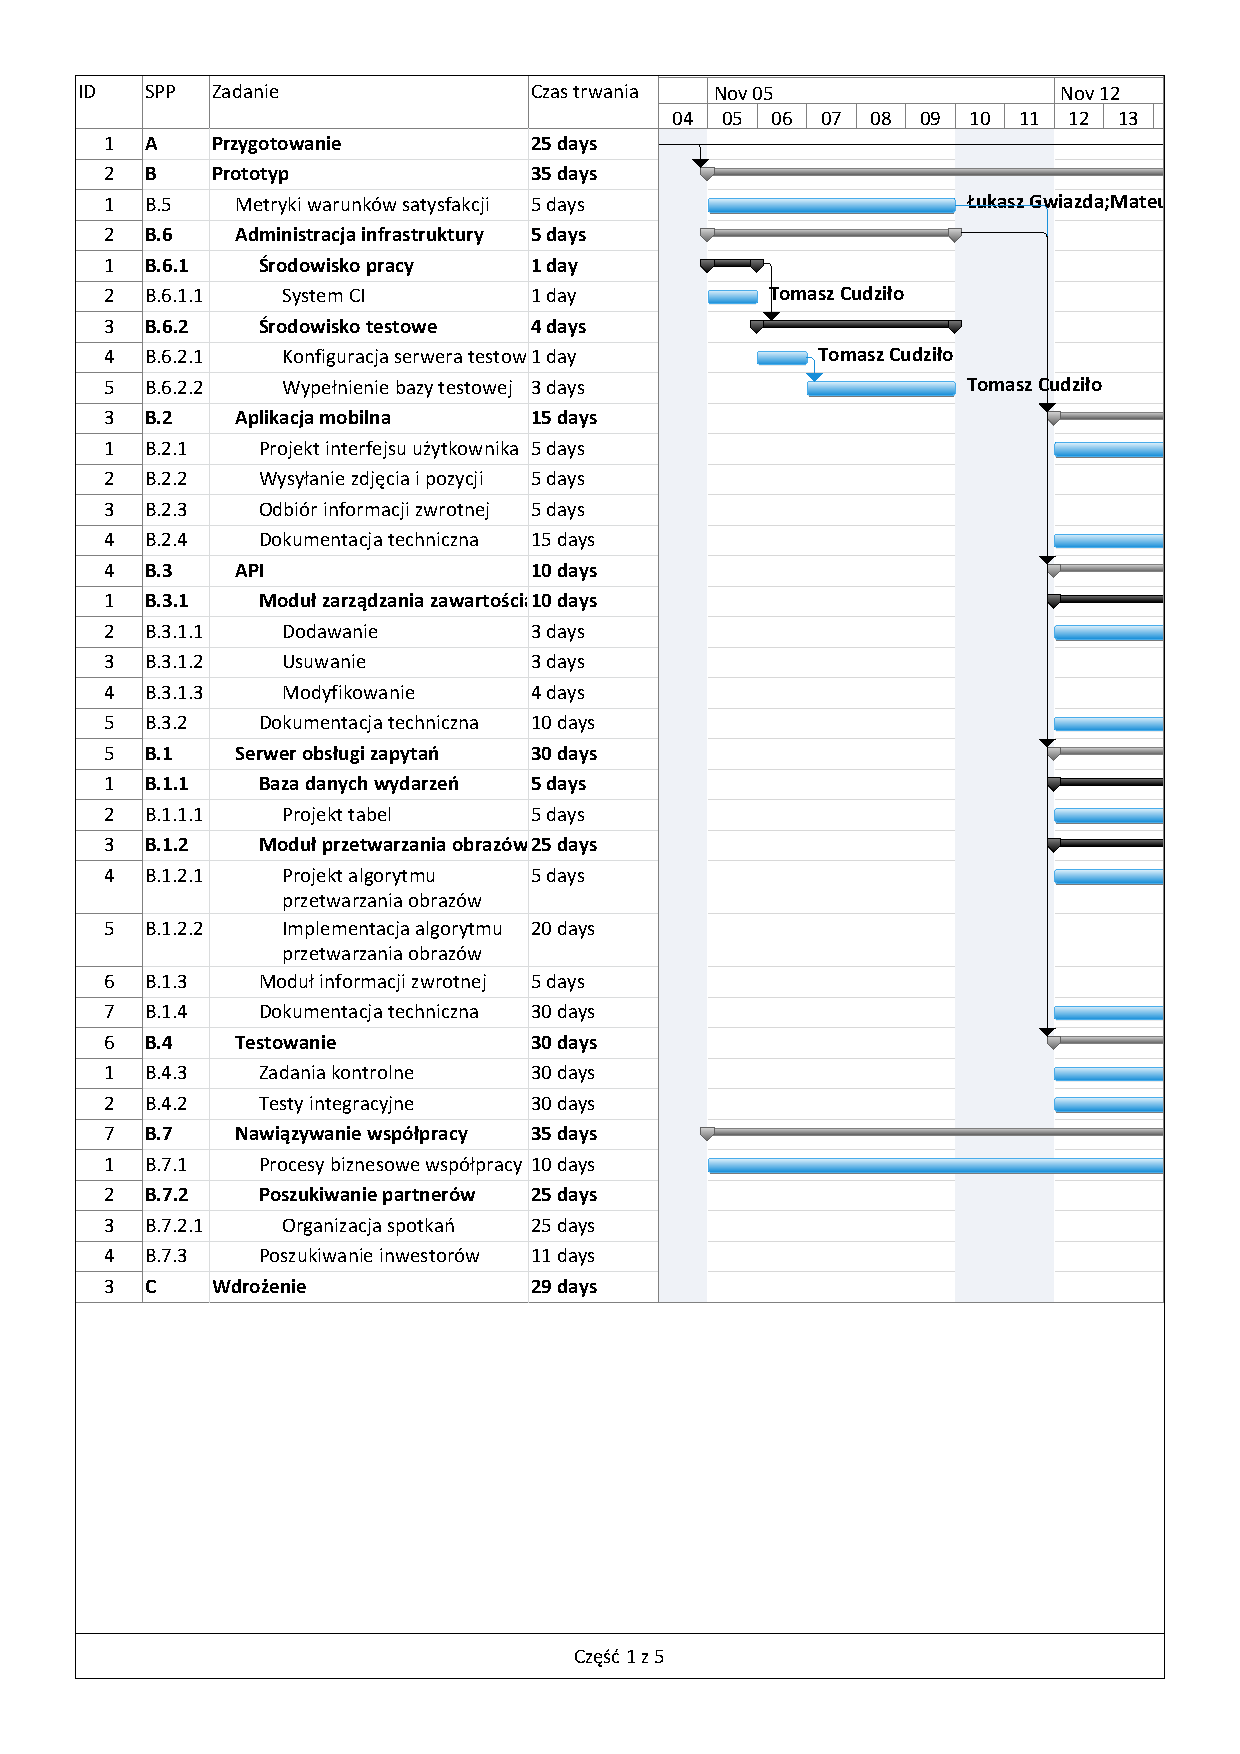
\includegraphics[trim=1.2cm 1.2cm 1.2cm 1.2cm, page=1, width=\textwidth]{./figury/organizacja-pracy-B-prototyp}
    \caption{Harmonogram pracy iteracji \emph{Protyp} projektu \emph{Concerto}.}
    \label{fig:iteracja-prototyp}
\end{figure}

\begin{figure}[p]
    \ContinuedFloat
    \includegraphics[trim=1.2cm 1.2cm 1.2cm 1.2cm, page=2, width=\textwidth]{./figury/organizacja-pracy-B-prototyp}
    \caption[]{Harmonogram pracy iteracji \emph{Prototyp} projektu \emph{Concerto}. (kontynuacja)}
\end{figure}

\begin{figure}[p]
    \ContinuedFloat
    \includegraphics[trim=1.2cm 1.2cm 1.2cm 1.2cm, page=3, width=\textwidth]{./figury/organizacja-pracy-B-prototyp}
    \caption[]{Harmonogram pracy iteracji \emph{Prototyp} projektu \emph{Concerto}. (kontynuacja)}
\end{figure}

\begin{figure}[p]
    \ContinuedFloat
    \includegraphics[trim=1.2cm 1.2cm 1.2cm 1.2cm, page=4, width=\textwidth]{./figury/organizacja-pracy-B-prototyp}
    \caption[]{Harmonogram pracy iteracji \emph{Prototyp} projektu \emph{Concerto}. (kontynuacja)}
\end{figure}

\begin{figure}[p]
    \ContinuedFloat
    \includegraphics[trim=1.2cm 1.2cm 1.2cm 1.2cm, page=5, width=\textwidth]{./figury/organizacja-pracy-B-prototyp}
    \caption[]{Harmonogram pracy iteracji \emph{Prototyp} projektu \emph{Concerto}. (kontynuacja)}
\end{figure}

\subsection{Iteracja C -- Wdrożenie}

Harmonogram prac wchodzących w skład iteracji \emph{Wdrożenie}
zaczyna się na stronie \pageref{fig:iteracja-wdrozenie}.

\begin{figure}[p]
    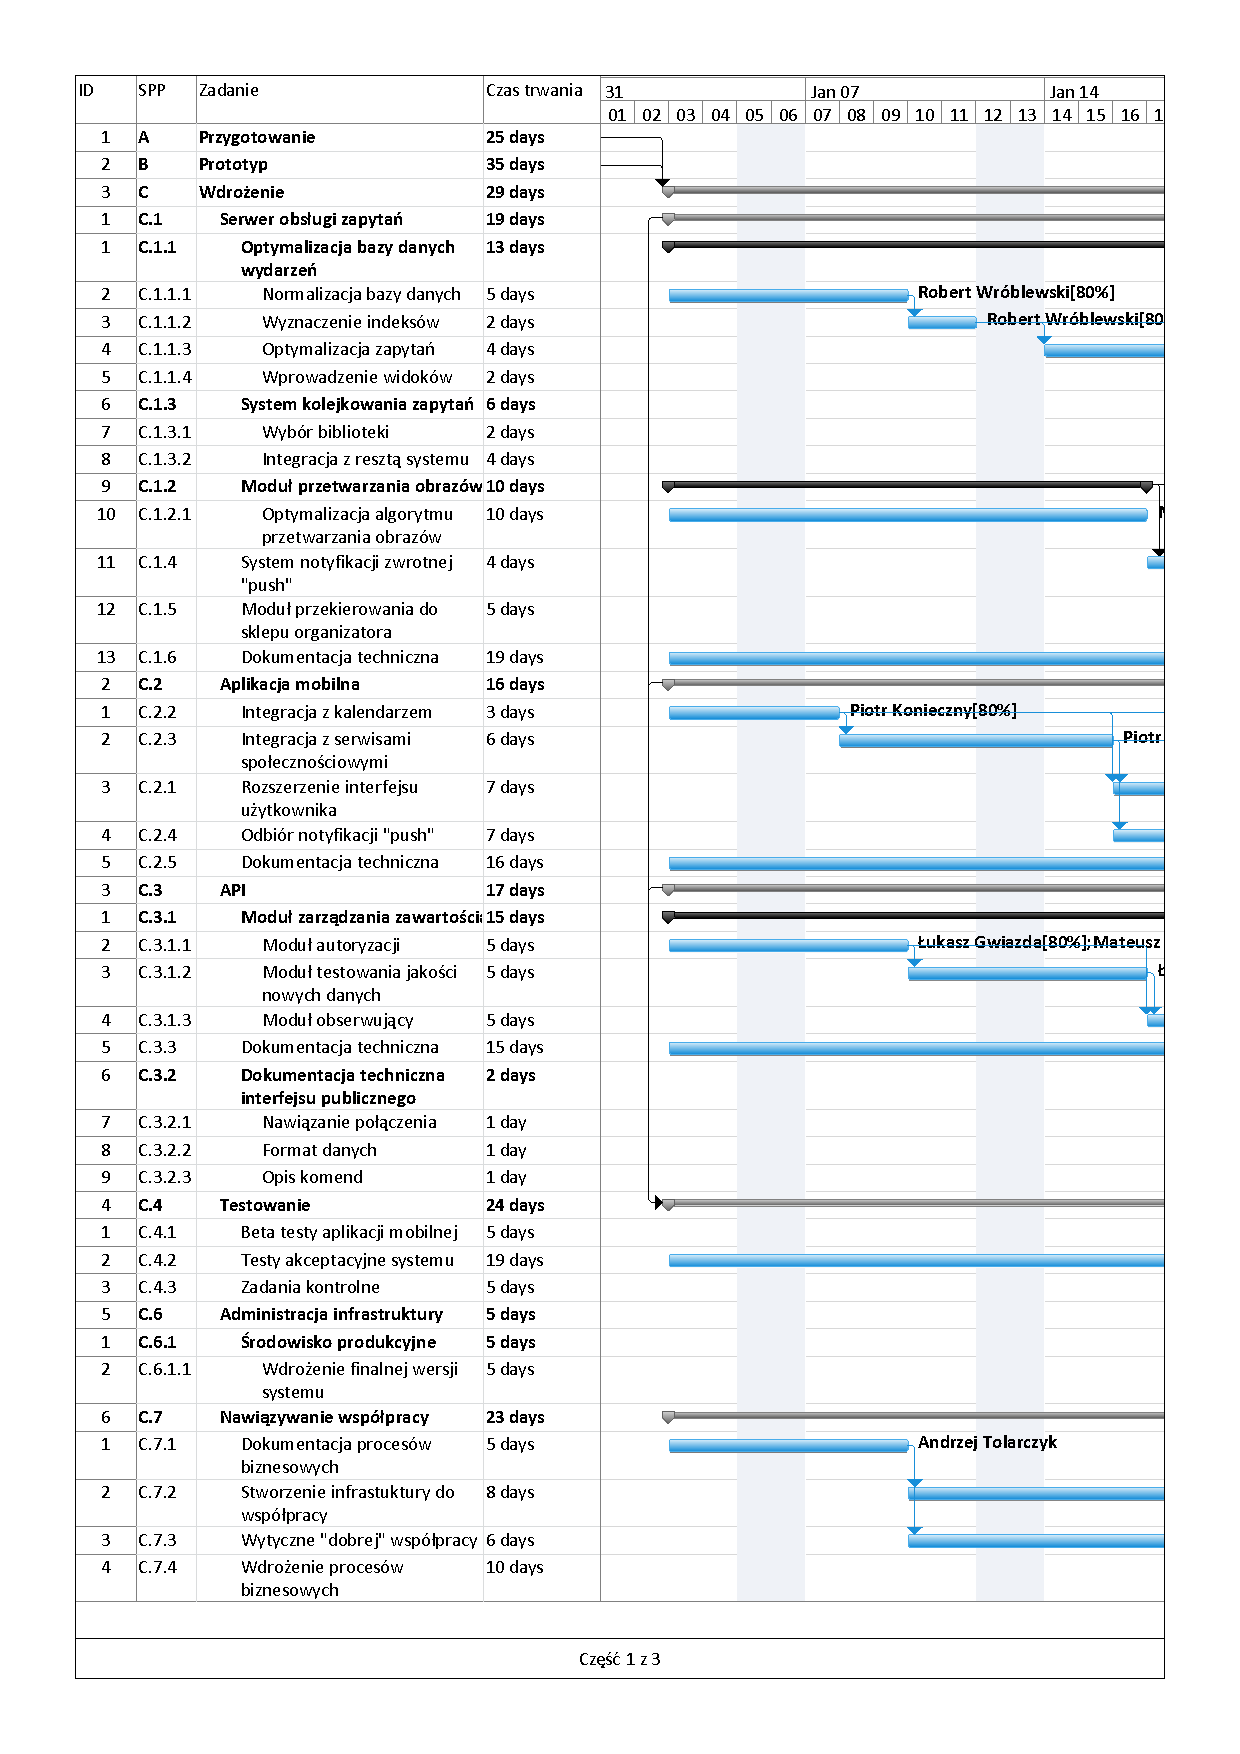
\includegraphics[trim=1.2cm 1.2cm 1.2cm 1.2cm, page=1, width=\textwidth]{./figury/organizacja-pracy-C-wdrozenie}
    \caption{Harmonogram pracy iteracji \emph{Wdrożenie} projektu \emph{Concerto}.}
    \label{fig:iteracja-wdrozenie}
\end{figure}

\begin{figure}[p]
    \ContinuedFloat
    \includegraphics[trim=1.2cm 1.2cm 1.2cm 1.2cm, page=2, width=\textwidth]{./figury/organizacja-pracy-C-wdrozenie}
    \caption[]{Harmonogram pracy iteracji \emph{Wdrożenie} projektu \emph{Concerto}. (kontynuacja)}
\end{figure}

\begin{figure}[p]
    \ContinuedFloat
    \includegraphics[trim=1.2cm 1.2cm 1.2cm 1.2cm, page=3, width=\textwidth]{./figury/organizacja-pracy-C-wdrozenie}
    \caption[]{Harmonogram pracy iteracji \emph{Wdrożenie} projektu \emph{Concerto}. (kontynuacja)}
\end{figure}


\section{Historia dokumentu}
\begin{versions}
    \version*{0.1}{2012-11-24}{TC}%
        Dodano podział na iteracje i zadania do 2. poziomu WBS.
    \version{0.2}{2012-11-27}{MO}%
        Dodano zadania do 3. poziomu WBS.
    \version{0.3}{2012-11-28}{MM}%
        Przypisano zasoby i wyważono rozkład zadań pomiędzy pracowników.
    \version{0.4}{2012-11-29}{TC,MM,MO}%
        Linearyzowanie pracy, prewencja długich okresów bez przypisanych zadań.
    \version{0.5}{2012-11-29}{MM,MO}%
        Finalne poprawki wizualne i merytoryczne.
    \version{1.0}{2012-11-30}{TC}%
        Zatwierdzenie dokumentu.
\end{versions}


\end{document}
